\documentclass[twoside,11pt]{article}

%%%%% PACKAGES %%%%%%
\usepackage{pgm2016}
\usepackage{amsmath}
\usepackage{algorithm}
\usepackage[noend]{algpseudocode}
\usepackage{subcaption}
\usepackage[utf8]{inputenc}		%NOT USED?
\usepackage[english]{babel}		%NOT USED?
\usepackage{paralist}			%NOT USED?
\usepackage[lowtilde]{url}
\usepackage{fixltx2e}
\usepackage{listings}
\usepackage{color}
\usepackage{hyperref}



%%%%% MACROS %%%%%%
\algrenewcommand\Return{\State \algorithmicreturn{} }
\algnewcommand{\LineComment}[1]{\State \(\triangleright\) #1}
\renewcommand{\thesubfigure}{\roman{subfigure}}
\definecolor{codegreen}{rgb}{0,0.6,0}
\definecolor{codegray}{rgb}{0.5,0.5,0.5}
\definecolor{codepurple}{rgb}{0.58,0,0.82}
\definecolor{backcolour}{rgb}{0.95,0.95,0.92}
\lstdefinestyle{mystyle}{
   backgroundcolor=\color{backcolour},  
   commentstyle=\color{codegreen},
   keywordstyle=\color{magenta},
   numberstyle=\tiny\color{codegray},
   stringstyle=\color{codepurple},
   basicstyle=\footnotesize,
   breakatwhitespace=false,        
   breaklines=true,                
   captionpos=b,                    
   keepspaces=true,                
   numbers=left,                    
   numbersep=5pt,                  
   showspaces=false,                
   showstringspaces=false,
   showtabs=false,                  
   tabsize=2
}
\lstset{style=mystyle}

%%%%% SHORT HEADING %%%%%%
% Short headings should be running head and authors last names
\ShortHeadings{Research Task B - The Platform: Wit.ai}{dos Santos}
\firstpageno{1}

\begin{document}

\title{The Platform: Wit.ai}

\author{\name André E. dos Santos \email dossantos@cs.uregina.ca \\
\addr Department of Computer Science \\
University of Regina \\ 
Regina, Canada
}



\maketitle

\begin{abstract}%   <- trailing '%' for backward compatibility of .sty file
\emph{Wit.ai} is \emph{cloud service} that turns speech or text into actionable data.
Wit is supported on every major platform and can be implemented in mobile apps, home automation, wearable devices, robots, and messenger agents.
Thus, it is a interesting \emph{natural language processing} tool for developers.

In this paper we give a introduction on how to create a Wit.ai app.
We show how to add Wit to a web app and use the actionable data to change the colour of an object on the webpage ``on the fly.''
The result is an interactive webpage the ``understands'' the user.
Although being a simple application, it shows how Wit can be implemented and collaborate with different type of resources.
\end{abstract}


%\begin{lstlisting}[language=bash]
%mkdir folder
%\end{lstlisting}

\section{Introduction}
\label{sec:intro}

\emph{Natural language processing} is the technology for dealing with a variety of human language in thousands of languages and varieties \citep{jurafsky2014speech}. 
Since the last decade, every year we seem more of successful natural language processing applications on our day-by-day.
Spelling and grammar correction in word processors, machine translation on the web, and email spam detection are some of the many applications of natural language processing that are present on our most common daily routine.
Observing this potential, the online social networking service \emph{Facebook} acquired \cite{1_wit.ai_2016}, a startup founded to create an API for building voice-activated interfaces. 

With only a few lines of its code, Wit.ai let developers build a speech recognition and voice control console.
Wit does not require expertise in natural language processing from the developers.
Thus, it can save time and resources which would be required to build even the simplest voice-recognition system.
To build a voice application in Wit it is necessary to determine intents and then training the app to improve its accuracy.
Wit has a friendly interface, making the process of training quickly and easy.

In this paper we implement a Wit app and show all steps of its precesses.
The objective of our application is to get colour information from voice recognition and change a \emph{html} object with this colour ``on the fly.''
The result is one of Wit many applications with an interactive webpage that ``understand'' voice commands and modify its object according to them.


This paper is organized as follows.
Section \ref{sec:get} presents the steps to create a application of Wit.
A web application with Wit is given in Section \ref{sec:web}.
Conclusions are drawn in Section \ref{sec:conc}.

\section{Getting Started}
\label{sec:get}


In this section, we demonstrate the steps to build a voice application on Wit.ai that obtains colour information from voice recognition and changes one html object with it ``on the fly.''
Note that, in order to sign up on Wit.ai and create the voice application, Wit only allow access through a \cite{github_2016} account.


\subsection{The Console}

Once with access to Wit.ai, one is already able to access to what is called the Wit Console. 
The Console is where we can manage the Wit.ai-powered apps, configure a voice app and improve it.
Thus, on the Wit Console App is where the voice applications logic abides.
For instance, the Wit Console with Apps $HelloWorld$ and $ColourTest$ is shown in Figure \ref{fig:console}.
Note that if a user signs in for the first time, Wit.ai creates the first app and the user will land on its page.
We can create new apps from the top-right menu.

\begin{figure}
\label{fig:console}
\centerline{
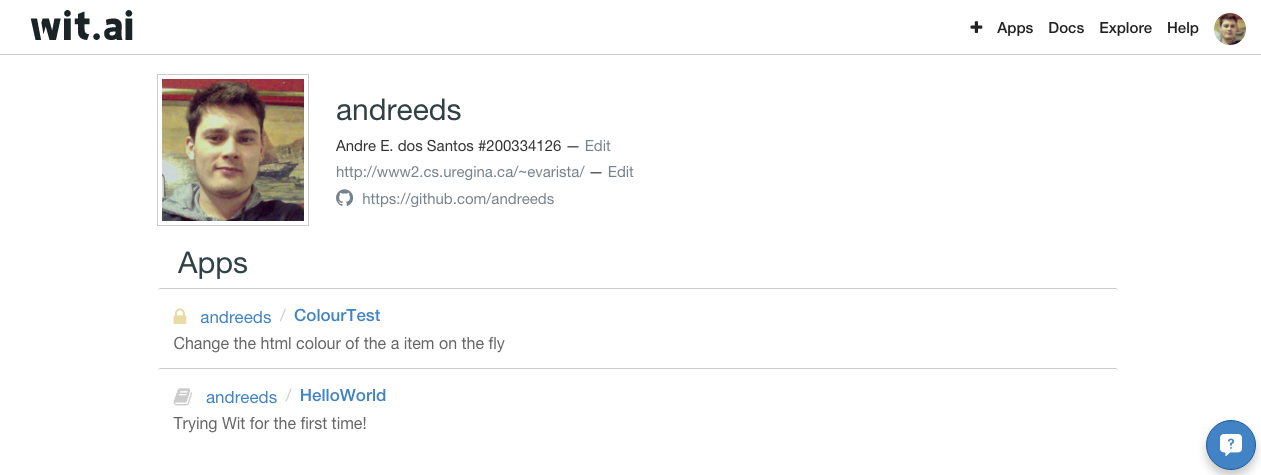
\includegraphics[width=\textwidth]{figures/Wit_Console.png}
}
\caption{The Wit Console.}
\end{figure}

\subsection{Determining and Creating User Intent}

Given that the user has created a new app, it is time to determine the its intents.
An intent is something that the end-user wants to perform.
For example,
``ask about the weather'', 
``set an alarm on their smartwatch'', and 
``say hello to their robot''.
It is common to focus on a finite list of possible intents.
Hence, each intent corresponds to one action in the app.
For our application, the intent is to ``change the colour of the object'' and also``greetings.''

Once with a raw speech or text input, Wit.ai will determine what is the user intent.

\begin{example}
\label{exe:intent}
All the following expressions should be mapped to the same intent:
\begin{lstlisting}[language=html]
``Change the colour to red''
``Colour: red''
``I want the colour to be red''
\end{lstlisting}
\end{example}

There are many different ways to express the same intents. 
Thus, it is the job of Wit.ai to map these expressions to actual intents.

The user can browse existing intents from the community of Wit online.
When typing examples for the intents, Wit will suggest these existing intents. 
It is optional to browse the suggested intents and check  if one fits the current intent. 
If so, clicking on “GET” will get a copy of the existing intent in the Wit app.
If not, it is necessary to create a new intent.

To create a new intent, type a name for your new intent in the Name your intent field.
Usually, intent names try to match the app functions or methods. 
Add at least three expressions, even with synonymous way to say the same command.
Figure \ref{fig:entents} shows the intents $colour$ and $greeting$ for the ColourTest App.
Some of the expressions for $colour$ is listed in Example \ref{exe:intent}.


\begin{figure*}[!h]
    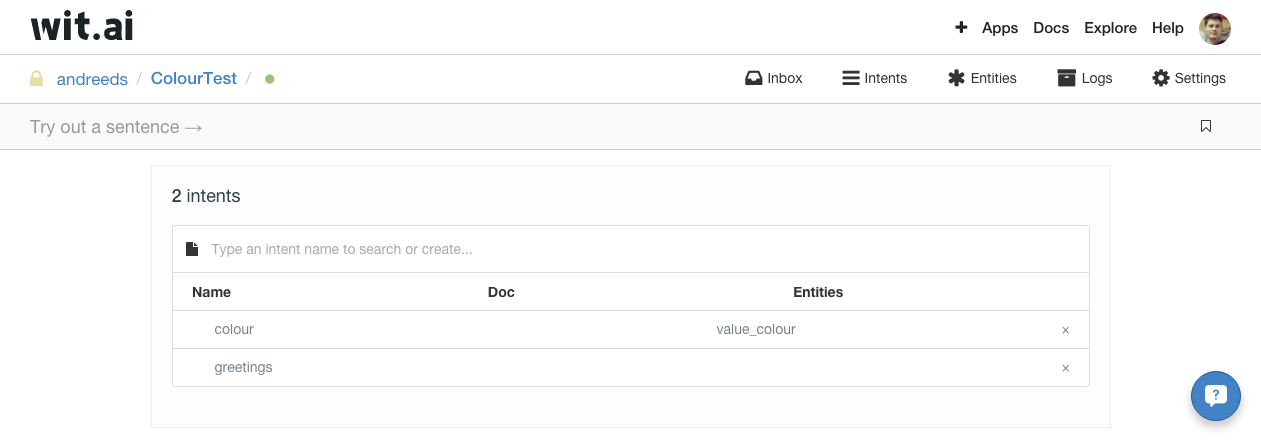
\includegraphics[width=\textwidth]{figures/entities.png}
    \caption{The intents for the ColourTest App.}
    \label{fig:entents}
\end{figure*}


\subsection{Training}

It is time to query the voice app.
At this point, we can already request the voice app via the Wit.ai API.

Notice that, before trainig the app, it is necessary to add the \emph{Client Access Token} to the website.
We will show more details about this step in Section \ref{sec:web}.

In the Inbox of the App we can see the examples said when inputed troght website.

\subsubsection{Validate Audio from the Inbox}

At Inbox we can validate the the correct sentences recorded by Wit.
Once trained, Wit improves its speech recognitions an the \emph{Confidence} ratio for the expression intents tends to raise.
To train the voice is very simple.
For each expression it reproduces the audio recorded.
If it is correct, we can validate it.
If not, we type the correct sentence and then validate it.

\subsubsection{Validate Expressions from the Inbox}


At Inbox we can validate matches with expression and intents that were correctly captured by Wit.
For instance, Figure \ref{fig:expressions} shows three expressions captured by Wit, the first one was validated as intent $greetings$, the second was \emph{Archived} since was any of the existing intents, and the third one was validated as intent $colour$.
In our example, we also want to capture the targeted colour.
This is called an \emph{Entity}. 
We can create our own one or select a common one from the dropdown list. 
For instance, the entity $value\_colour$ was created for the intent $colour$, as depicted in Figure \ref{fig:expressions} bottom.


\begin{figure*}[!h]
\begin{center}
    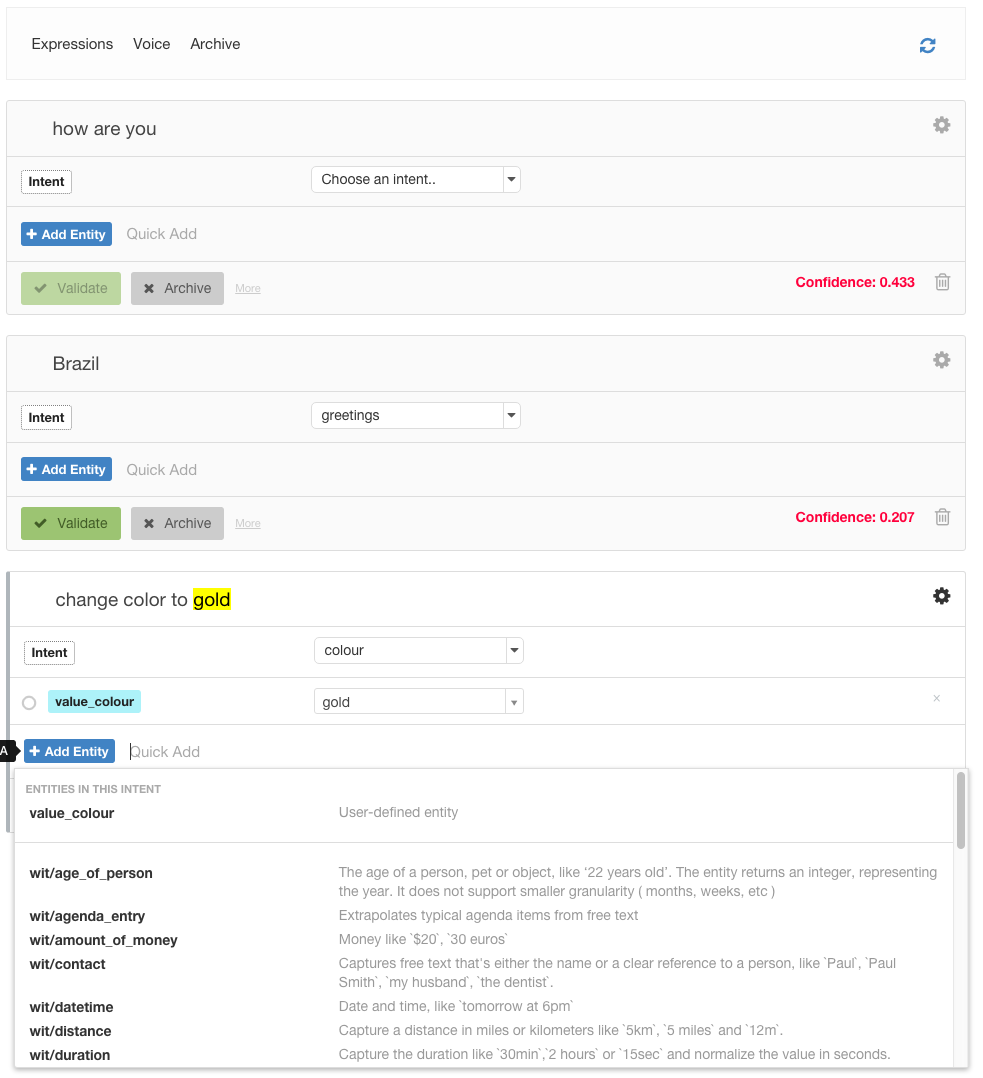
\includegraphics[width=0.75\textwidth]{figures/expressions.png}
    \caption{Expressions captured by Wit.ai.}
    \label{fig:expressions}
\end{center}
\end{figure*}

\section{Web application}
\label{sec:web}

Now we show how to add Wit to a web app.
As a prerequisites, the browser must support \cite{webrtc}, which is the case of Chrome, Firefox and Opera.

To integrate the voice app with the web app we need to create a new folder for the app, download the Web SDK (aka. Microphone) and extract the archive:
\begin{lstlisting}[language=bash]
	mkdir myapp
	cd myapp
	curl -L <https://github.com/wit-ai/microphone/releases/download/0.7.0/microphone-0.7.0.tar.gz | tar xvzf -
	mv microphone-* microphone
\end{lstlisting}

In the myapp folder, we must create a file $index.html$ containing the html provided by Wit on \url{https://wit.ai/docs/web/0.7.0}.

In the Setting page of the voice app we generate a \emph{Client Access Token}, as illustrated in Figure \ref{fig:token} 
A client access token is unique and authorizes the domain to access the voice app. 
To use the client access token we must replace $CLIENT\_TOKEN$ on the $index.html$ file.
\begin{lstlisting}[language=java]
	mic.connect("AWRBY6WLIPAQP7PGCGMQQKKO45LELCWO");
\end{lstlisting}


\begin{figure*}[!h]
\begin{center}
    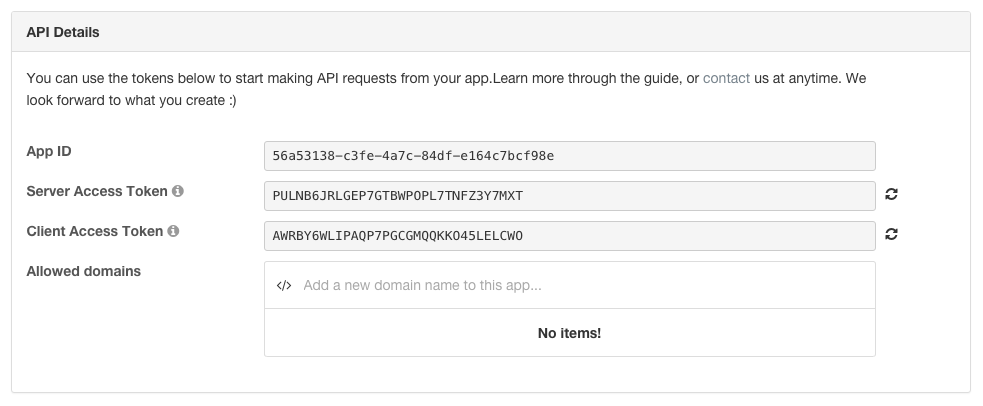
\includegraphics[width=0.75\textwidth]{figures/token.png}
    \caption{A Client Access Token.}
    \label{fig:token}
\end{center}
\end{figure*}


\subsection{In Action}

To see the web application in action we serve the app with a webserver.
For instance, using Python:
\begin{lstlisting}[language=bash]
	python -m SimpleHTTPServer
\end{lstlisting}
Then, to load the page on the browser
\begin{lstlisting}[language=bash]
	http://localhost:8000
\end{lstlisting}



After allowing your microphone, we will be able to click on the microphone icon and say a command. 
The command will be streamed to the voice app.

\subsection{Going Beyond}

At this point, our Wit app can already distinguish between intents and for the specific intent $colour$ it can capture its value.
To go beyond, we will use these informations to change an object on the webpage.
More specifically the circle:
\begin{lstlisting}[language=html]
	<svg height="150" width="150">
		<circle id="circle" cx="75" cy="75" r="50" stroke="#b2b2b2" stroke-width="4"/>
	</svg> 
\end{lstlisting}

To accomplish the objective we must add a conditional rule on \emph{javascript} \citep{flanagan2006javascript}: 
\begin{lstlisting}[language=java]
	if (intent == "colour"){
		cc(entities.value_colour.value);
 	}
\end{lstlisting}
so when intent $colour$ is observed, the circle $fill$ attribute changes to its value:
\begin{lstlisting}[language=java]
	function cc (j) {
		document.getElementById("circle").setAttribute("fill", j);

	}
\end{lstlisting}

The function $cc$ changes the attribute $fill$ of the circle created.
Thus, it can be called to also display a different colour when the mic is recording:
\begin{lstlisting}[language=java]
	mic.onaudiostart = function () {
		info("Recording started");
        error("");
        cc("red");
\end{lstlisting}

And, a response for $greetings$ can be given by:
\begin{lstlisting}[language=java]
	if (intent == "greetings"){
	document.getElementById("greet").innerHTML = "Hi :)";
	}
\end{lstlisting}

As a result, on the webpage the colour of the object changes according to the user's will using a voice command, as seen in Figure \ref{fig:webwit} (\subref{fig:colour}).
The website also recognizes when greeted, and it will reply back with the sentence``Hi :)'', as depicted in Figure \ref{fig:webwit} (\subref{fig:greeting}).


\begin{figure}[h]
\begin{center}
	\begin{subfigure}[t]{0.48\columnwidth}
	\begin{center}
   		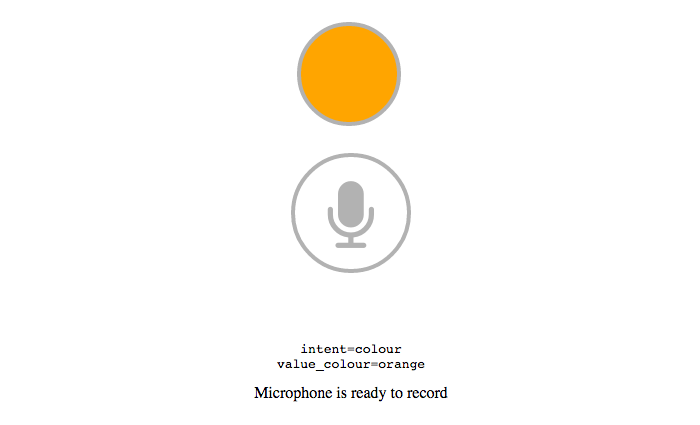
\includegraphics[width=\columnwidth]{figures/witapp_colour.png}
   		\caption{}
   		\label{fig:colour}
   	\end{center}
   \end{subfigure}
   \hfill
   \begin{subfigure}[t]{0.48\columnwidth}
	\begin{center}
   		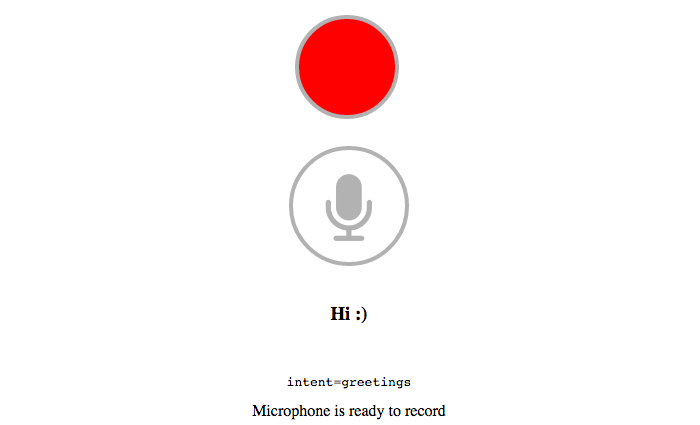
\includegraphics[width=\columnwidth]{figures/witapp_greetings.png}
   		\caption{}
   		\label{fig:greeting}
   	\end{center}
   \end{subfigure}
    \caption{A Client Access Token.}
    \label{fig:webwit}
\end{center}
\end{figure}


The complete code can be found on the GitHub repository on this \href{https://github.com/andreeds/cs807-research-tasks/tree/master/B\%20-\%20The\%20Platform/Wit}{link}.

\section{Conclusion}
\label{sec:conc}

Wit.ai is a cloud service that allows a simple implementation of natural language processing for developers.
With only a few lines of its code, Wit.ai let developers build a speech recognition and voice control console.
Thus, Wit has potential for many applications.
In this paper we demonstrated an application of Wit.
Using the speech recognition tool of Wit, we could change the colour of an html object on real time as well responding to greetings: a webpage that interacts with the user.






\vskip 0.2in
\bibliography{references/references}
\end{document}
